\Authors{Note that it is not clear at the moment if the ideas of \cref{sec:mainideas} work as intended.}
In this section we sketch a termination analysis and its soundness proof for languages with data and pattern matching as well as codata and copattern matching.
\\
First note that, according to the difference of natural deduction and sequent calculus there are two ways to formulate such a language.
The natural deduction formulation is biased towards producers (that is, proofs) whereas the sequent calculus formualtion refines and generalizes the natural deduction formulation by being symmetric in producers and consumers (that is, proofs and refutations).
This in particular means that one can translate semantic-preservingly from the producer-biased calculus to the symmetric calculus (\cref{sec:mainideas:calculi}).
Hence a termination analysis of the latter does also apply to the former and it suffices to examine termination in the latter case.
\\
The idea for our termination analysis then is to instantiate the size-change termination principle (\cref{sec:mainideas:sctp}) with strict positivity (\cref{sec:mainideas:sp}) and structural recursion (\cref{sec:mainideas:sr}), mirroring the usual ones for data with pattern matching (\cite{pauline-mohring}, \cite{foetus} and \cite{abel-altenkirch}).
The soundness proof (\cref{sec:mainideas:sound}) leverages information which are implicit in the procuder-biased calculus but explicit in the symmetric calculus.
\\
In the following we discuss the ideas of the aformentioned cornerstones on an intuitive level before working out the details in \cref{sec:formalization}.

\subsection{The Calculi}
\label{sec:mainideas:calculi}
\Authors{Turn the skeleton of \cref{sec:mainideas:calculi} into a nice text describing the languages and the translation.}

Let us first discuss the involved calculi and how to translate between them.

\subsubsection{Producer-Biased Calculus (PBC)}

The PBC is essentially the language presented in \cite{uroboro}.
One can consider it a subset of Agda.
Typical examples can be found in \cref{fig:mainideas:PBC:type}.

\begin{figure}[h]
  \begin{subfigure}[b]{0.3\textwidth}
    \begin{codealign}
      % Nat datatype
      &
        \data\ \Nat\ \where
      \\[-4pt]
      &\quad
        \Zero : \Nat
      \\[-4pt]
      &\quad
        \Succ(n : \Nat) : \Nat
      \\
      % addition function
      &
        \define\
        \Nat.\plus(m : \Nat) : \Nat
        \coloneq
        \match
      \\[-4pt]
      &\quad
        \Zero \Rightarrow m
      \\[-4pt]
      &\quad
        \Succ(n : \Nat) \Rightarrow n.\plus(\Succ(m))
    \end{codealign}
    \caption{Inductive Type.}
    \label{fig:mainideas:PBC:type:inductive}
  \end{subfigure}
  \begin{subfigure}[b]{0.3\textwidth}
    \begin{codealign}
      % FunNatNat codatatype
      &
        \codata\ \FunNatNat\ \where
      \\[-4pt]
      &\quad
        \FunNatNat.\Apply(n : \Nat) : \Nat
      \\
      % identity function
      &
        \define\
        \id : \FunNatNat
        \coloneq
        \comatch
      \\[-4pt]
      &\quad
        \Apply(n : \Nat) \Rightarrow n
      \\
    \end{codealign}
    \caption{Function Type.}
    \label{fig:mainideas:PBC:type:function}
  \end{subfigure}
  \begin{subfigure}[b]{0.35\textwidth}
    \begin{codealign}
      % StreamNat codatatype
      &
        \codata\ \StreamNat\ \where
      \\[-4pt]
      &\quad
        \StreamNat.\Head : \Nat
      \\[-4pt]
      &\quad
        \StreamNat.\Tail : \StreamNat
      \\
      % constant function
      &
        \define\
        \const(n : \Nat) : \StreamNat
        \coloneq
        \comatch
      \\[-4pt]
      &\quad
        \Head \Rightarrow n
      \\[-4pt]
      &\quad
        \Tail \Rightarrow \const(n)
    \end{codealign}
    \caption{Coinductive Type.}
    \label{fig:mainideas:PBC:type:coinductive}
  \end{subfigure}
  \caption{Examples of types in PBC.}
  \label{fig:mainideas:PBC:type}
\end{figure}

Terms $t$ of the PBC are either variables $x$ or producer applications $\mathcal{C}\overline{t}$ or consumer applications $t.\mathcal{D}\overline{t}$.
For more details see \cref{sec:formalization}.

In the PBC, a \textit{call} is the application of a
\begin{enumerate}
  \item
    match $t.\mathcal{D}\overline{t}$
  \item
    comatch $\mathcal{C}\overline{t}$
\end{enumerate}
to terms $t$.
Examples for calls are
\begin{enumerate}
  \item
    $\Zero.\plus(\Succ(\Zero))$ (evaluating to $\Succ(\Zero)$)
  \item
    $\id().\Apply(\Zero)$ (evaluating to $\Zero$)
  \item
    $\const(\Zero).\Head()$ (evaluating to $\Zero$)
\end{enumerate}
Moreover, the \textit{body} of a
\begin{enumerate}
  \item
    match associated with a constructor $\mathcal{C}$
  \item
    comatch associated with a destructor $\mathcal{D}$
\end{enumerate}
is the term $t$ related to it by $\Rightarrow$ in the definition.
For example, the body of $\plus$ associated with $\Zero$ is $m$ while the body of $\const$ w.r.t. $\Tail$ is $\const(n)$.

\subsubsection{Symmetric Calculus (SC)}

The SC is essentially the PBC with natural deduction style replaced by sequent calculus style.
This manifests itself most obviously in the refinement of the typing judgement: instead of only $\typetmpbc{\Gamma}{t}{T}$ ($t$ has type $T$) one has $\typetmprd{\Gamma}{t}{T}$ ($t$ is a producer of $T$) and $\typetmcon{\Gamma}{t}{T}$ ($t$ is a consumer of $T$).
Then a producer can be \enquote{cut} with a consumer of the same type to form a command spawning a computation.
Examples corresponding to the typical ones of the PBC \cref{fig:mainideas:PBC:type} can be found in \cref{fig:mainideas:SC:type}.

\begin{figure}[h]
  \begin{subfigure}[b]{0.3\textwidth}
    \begin{codealign}
      % Nat datatype
      &
        \polprd\ \type\ \Nat\ \where
      \\[-4pt]
      &\quad
        \Zero
      \\[-4pt]
      &\quad
        \Succ(n \prd \Nat)
      \\
      % addition function
      &
        \define\
        \plus(m \prd \Nat, k \con \Nat) \con \Nat
        \coloneq
        \match
      \\[-4pt]
      &\quad
        \Zero \Rightarrow m \mkCmd k
      \\[-4pt]
      &\quad
        \Succ(n \prd \Nat) \Rightarrow n \mkCmd \plus(\Succ(m), k)
    \end{codealign}
    \caption{Inductive Type.}
    \label{fig:mainideas:SC:type:inductive}
  \end{subfigure}
  \begin{subfigure}[b]{0.3\textwidth}
    \begin{codealign}
      % FunNatNat codatatype
      &
        \polcon\ \type\ \FunNatNat\ \where
      \\[-4pt]
      &\quad
        \Apply(n \prd \Nat, k \con \Nat)
      \\
      % identity function
      &
        \define\
        \id \prd \FunNatNat
        \coloneq
        \match
      \\[-4pt]
      &\quad
        \Apply(n \prd \Nat, k \con \Nat) \Rightarrow n \mkCmd k
      \\
    \end{codealign}
    \caption{Function Type.}
    \label{fig:mainideas:SC:type:function}
  \end{subfigure}
  \begin{subfigure}[b]{0.35\textwidth}
    \begin{codealign}
      % StreamNat codatatype
      &
        \polcon\ \type\ \StreamNat\ \where
      \\[-4pt]
      &\quad
        \Head(k \con \Nat)
      \\[-4pt]
      &\quad
        \Tail(k \con \StreamNat)
      \\
      % constant function
      &
        \define\
        \const(n \prd \Nat) \prd \StreamNat
        \coloneq
        \match
      \\[-4pt]
      &\quad
        \Head(k \con \StreamNat) \Rightarrow n \mkCmd k
      \\[-4pt]
      &\quad
        \Tail(k \con \StreamNat) \Rightarrow \const(n) \mkCmd k
    \end{codealign}
    \caption{Coinductive Type.}
    \label{fig:mainideas:SC:type:coinductive}
  \end{subfigure}
  \caption{Examples of types in SC.}
  \label{fig:mainideas:SC:type}
\end{figure}

Terms $t$ of the SC are either variables $x$ or applications $\mathcal{X}\overline{t}$.
For more details see \cref{sec:formalization}.

In the SC, a \textit{call} is the application of a match $\mathcal{X}$
\begin{enumerate}
  \item
    in consumer position of a command $\ldots \mkCmd \mathcal{X}\ldots$
  \item
    in producer position of a command $\mathcal{X}\ldots \mkCmd \ldots$
\end{enumerate}
Examples for calls are
\begin{enumerate}
  \item
    $\Zero \mkCmd \plus(\Succ(\Zero), k)$ (reducing to $\Succ(\Zero) \mkCmd k$)
  \item
    $\id() \mkCmd \Apply(\Zero, k)$ (reducing to $\Zero \mkCmd k$)
  \item
    $\const(\Zero) \mkCmd \Head(k)$ (reducing to $\Zero \mkCmd k$)
\end{enumerate}
Moreover, the \textit{body} of a match associated with a 
\begin{enumerate}
  \item
    producer $\mathcal{X}$ of a $\polprd$ type
  \item
    consumer $\mathcal{X}$ of a $\polcon$ type
\end{enumerate}
is the command $c$ related to it by $\Rightarrow$ in the definition.
For example, the body of $\plus$ associated with $\Zero$ is $m \mkCmd k$ while the body of $\const$ w.r.t. $\Tail$ is $\const(n) \mkCmd k$.

\subsubsection{Translate from the PBC to the SC}
The translation is essentially a CPS transformation using continuation types of the form

\begin{codealign}
  % continuation datatype
  &
    \polcon\ \type\ \ContT\ \where
  \\[-4pt]
  &\quad
    \Jump(x \prd T)
\end{codealign}

and

\begin{codealign}
  % cocontinuation datatype
  &
    \polprd\ \type\ \CocontT\ \where
  \\[-4pt]
  &\quad
    \Cojump(k \con T)
\end{codealign}

for syntactically implicit control flow in the PBC.

\subsection{Size-Change Termination Principle (SCTP)}
\label{sec:mainideas:sctp}

The size change termination principle is a general approach to approxiamte a decision of termination for language constructs that operate on finitistically structured data.
\cite{lee + jones + ben-amran} introduced it on the basis of a language with functions operating on a domain which is assumed to be well-founded w.r.t. some order relation $<$.
The idea is that in any infinite sequence of function calls some function $f$ would have to occur infinitely often.
But if in each pair of successive calls of $f$ in such a sequence the argument becomes smaller w.r.t. $<$, the sequence could not have been infinite in the first place.
This is becasuse the arguments cannot decrease forever due to the well-foundedness of $<$.
That is, if $\evaluatesto^{\ast}$ denotes evaluation in perhaps several steps then
\begin{align*}
  f(x_{1})
  &\evaluatesto^{\ast}
  f(x_{2})
  \evaluatesto^{\ast}
  f(x_{3})
  \evaluatesto^{\ast}
  \ldots
  \\
  x_{1}
  &>
  x_{2}
  >
  x_{3}
  >
  \ldots
\end{align*}
is a contradiction due to the well-foundedness of $<$.
So the size change termination principle says that if a program tries to only decrease some finitistically structured datum infinitely often, then it terminates.
\\
To apply the principle to a language one has to structure the its data finitistically and ensure that the size of some datum is constantly reduced.
This works particular well for a language consisting of data types and pattern matching with mutual recursion excluded like the PBC restrcited to $\data$ and $\match$ with the respective restriction regarding mutuality.
Because then a $\data$ type is essentially a well-founded tree.
In that case, programs terminate if matches calling themselves have to do so on an argument which is smaller than the original.
\\
$\plus$ on $\Nat$ from \cref{fig:mainideas:PBC:type:inductive} is an archetypical example.
$\Succ(n).\plus(\ldots)$ calls $\plus$ but only on $n < \Succ(n)$ which is why it terminates.
\\
But in case of just streams \cref{fig:mainideas:PBC:type:coinductive} we can observe the size change principle, too: $\const$ calls itself lazily whenever a $\Head$ or $\Tail$ is applied to it but a programmer can only ever apply finitely many of them to destruct it.
The problem in a PBC-like setting is that regarding the typing judgement $\typetmpbc{\cdot}{\cdot}{\cdot}$ the codata is semantically not the observations constructed by $\Head$ and $\Tail$ but the streams.
And streams are non-wellfounded trees.
\\
This is different in an SC-like setting.
In \cref{fig:mainideas:SC:type:coinductive} the observations of streams are well-founded trees w.r.t. to the $\typetmcon{\cdot}{\cdot}{\cdot}$ judgement constituting the $\polcon$ type exactly in the same sense as natural numbers do in the $\polprd$ case.
\\
However, while well-foundedness seems clear in the case of isolated $\polprd$ and $\polcon$ types the general case of the SC is more complicated.
The mutuality allows for vicious circles which have to be excluded somehow.
\cref{sec:mainideas:sp} discusses how to do that using strict positivity restrictions.
Also, the size-decrease requirement needs a more sophisticated technique to exclude vicious circles originating in mutuality in the general case of the SC.
\cref{sec:mainideas:sr} discusses structural recursion in that regard.
\\
Finally, with strict positivity for the well-foundedness of the finitistically structured data ($\polprd$ and $\polcon$ types) and structural recursion for matches to ensure the correct size-changes in place we can discuss how to prove the SCTP for the SC sound in \cref{sec:mainideas:sr}.

\subsection{Strict Positivity}
\label{sec:mainideas:sp}

Famously, the Curry paradox $(X \Rightarrow Y) \Leftrightarrow X$ comprises the inconsistency that $X$ is false if and only if it is true: $(X \Rightarrow \bot) \Leftrightarrow X$.
This inconsistency also emerges in the Curry-Howard interpretation of logics allowing such a formulation in the guise of a certain kind of non-termination.
Strict positivity is a condition excluding that kind of non-termination by specifying which types are allowed on the left of $\rightarrow$.
\\
In the first part of this subsection we will consider the Curry-Paradox in the PBC and explain how to formulate strict positivity there to disarm Curry-like paradoxes.
Subsequently, this will guide the development of a strict positivity formualtion for the SC in the second part.

\subsubsection{PBC}

The PBC is based on a Curry-Howard interpretation and as such is susceptible to the Curry paradox.
\\
In that regard, first note that it is well-known that refutations $X \Rightarrow \bot$ become continuations $X \rightarrow \bot$ under the Curry-Howard interpretation and that function types are generalized by codata types.\footnote{Loosely speaking, one can consider codata as intensional definitions of recursive records of functions.}
\\
So to model the Curry paradox we can interpret $X \Rightarrow \bot$ as the codata type $\ContCurry$ with a destructor $\Jump$ from a type $\Curry$ interpreting $X$ to the empty type $\Empty$ interpreting $\bot$.
And as $\ContCurry$ types the continuations of $\Curry$, $\Curry$ has to consist of those.
That is, we can interpret $\Curry$ simply as the data type embedding $\ContCurry$ via a constructor $\MakeExe$.
\\
Given that model of the Curry paradox, it is not hard to write a non-terminating program without direct recursive calls in PBC: just define a continuation $\runarg$ running its argument where $\run$ning means to jump there with itself as argument.
Then, $\MakeExe(\runarg).\run()$ does not terminate.

\begin{minipage}{0.45\textwidth}
  \begin{codealign}
    % Curry datatype
    &
      \data\ \Curry\ \where
    \\[-4pt]
    &\quad
      \MakeExe(k : \ContCurry) : \Curry
    \\
    % run function
    &
      \define\
      \Curry.\run() : \Empty
      \coloneq
      \match
    \\[-4pt]
    &\quad
      \MakeExe(k : \ContCurry) \Rightarrow k.\Jump(\MakeExe(k))
    \\
  \end{codealign}
\end{minipage}
\begin{minipage}{0.45\textwidth}
  \begin{codealign}
    % ContCurry codatatype
    &
      \codata\ \ContCurry\ \where
    \\[-4pt]
    &\quad
      \Jump(x : \Curry) : \Empty
    \\
    % runarg function
    &
      \define\
      \runarg : \ContCurry
      \coloneq
      \comatch
    \\[-4pt]
    &\quad
      \Jump(x : \Curry) \Rightarrow x.\run()
    \\
  \end{codealign}
\end{minipage}

The culprit making the non-termination work is a malign circularity between $\Curry$ and $\ContCurry$ in analogy to the circularity in $(X \Rightarrow \bot) \Leftrightarrow X$ leading to an inconsitency.
If we didn't allow the type $\Curry$ in the domain of $\Jump$ in the first place, then we would not have been able to write that program.
The idea of strict positivity is to just exclude programs with that kind of circularity.
More precisely, strict positivity just prohibits circular occurences of a type on the left of an $\rightarrow$ or, more generally, circular occurences of a type in the domain of a destructor.
\\
This is still a somewhat vague formulation which has to be made even more precise to enable a real formalization, of course.
For that purpose one can use graphs to describe the type-structure of a program, allowing an easy formulation of strict positivity for PBC.
\\
To understand the type-structure of a program by means of graphs first note that a data type $T$ is declared with $n$ constructors named $\mathcal{C}_{1},\ldots,\mathcal{C}_{n}$ and domains (contexts) $\Delta_{1},\ldots,\Delta_{n}$ of which we can think of as a product of types here (see \cref{fig:mainideas:datatg:data}).
Likewise, a codata type $T$ is declared with $n$ destructors named $\mathcal{D}_{1},\ldots,\mathcal{D}_{n}$ additionally having codomains $T_{1},\ldots,T_{n}$ (see \cref{fig:mainideas:codatatg:codata}).
\\
So declaring types actually only involves saying how they relate to other types (including themselves and types declared at the same time).
The information for the data type in \cref{fig:mainideas:datatg:data} is still contained in the graph in \cref{fig:mainideas:datatg:tg} (where for a context $\Gamma$ we shall write $\#\vert \Gamma \vert$ for its total number of \enquote{factors} and $\Gamma(i)$ for the type in the $i$-th position).
The same holds for codata \cref{fig:mainideas:datatg:codata} with \cref{fig:mainideas:codatatg:tg}.
Sticking these building blocks together and perhaps bending the arrows to circles according to the the declarations in a program yields a directed graph with labeled arrows tracking the relations of types in the program.
We call this the \textit{type-graph} of the program.

\begin{figure}[h]
  \begin{subfigure}[b]{0.25\textwidth}
    \begin{codealign}
      % T datatype
      &
        \data\ T\ \where
      \\[-4pt]
      &\quad
        \mathcal{C}_{1} \Delta_{1} : T
      \\[-4pt]
      &\quad\quad\quad
        \vdots
      \\[-4pt]
      &\quad
        \mathcal{C}_{n} \Delta_{n} : T
    \end{codealign}
    \caption{Data declaration.}
    \label{fig:mainideas:datatg:data}
  \end{subfigure}
  \begin{subfigure}[b]{0.7\textwidth}
    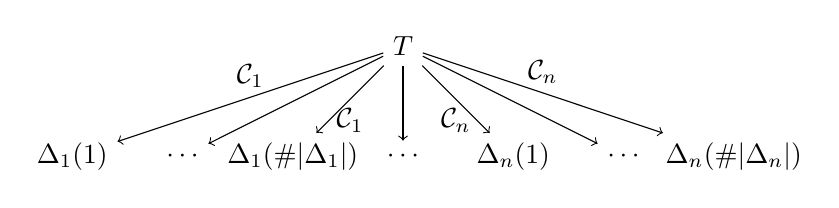
\begin{tikzpicture}[scale=0.7]
      % Nodes: types
      \node (T) at (0,2) { $T$  };
      \node (T1) at (-6,0) { $\Delta_{1}(1)$ };
      \node (Tcdots1) at (-4,0) { $\cdots$ };
      \node (T2) at (-2,0) { $\Delta_{1}(\#\vert \Delta_{1} \vert)$ };
      \node (Tcdots2) at (0,0) { $\cdots$ };
      \node (T3) at (2,0) { $\Delta_{n}(1)$ };
      \node (Tcdots3) at (4,0) { $\cdots$ };
      \node (T4) at (6,0) { $\Delta_{n}(\#\vert \Delta_{n} \vert)$ };
      % Arrows: level a to b
      \draw[solid,->] (T) -> (T1) node[midway,above] { $\mathcal{C}_{1}$ };
      \draw[solid,->] (T) -> (Tcdots1);
      \draw[solid,->] (T) -> (T2) node[midway,below] { $\mathcal{C}_{1}$ };
      \draw[solid,->] (T) -> (Tcdots2);
      \draw[solid,->] (T) -> (T3) node[midway,below] { $\mathcal{C}_{n}$ };
      \draw[solid,->] (T) -> (Tcdots3);
      \draw[solid,->] (T) -> (T4) node[midway,above] { $\mathcal{C}_{n}$ };
    \end{tikzpicture}
    \caption{Type-graph building block for data declaration.}
    \label{fig:mainideas:datatg:tg}
  \end{subfigure}
  \caption{Data.}
  \label{fig:mainideas:datatg}
\end{figure}

\begin{figure}[h]
  \begin{subfigure}[b]{0.3\textwidth}
    \begin{codealign}
      % T codatatype
      &
        \codata\ T\ \where
      \\[-4pt]
      &\quad
        T.\mathcal{D}_{1} \Delta_{1} : T_{1}
      \\[-4pt]
      &\quad\quad\quad
        \vdots
      \\[-4pt]
      &\quad
        T.\mathcal{D}_{n} \Delta_{n} : T_{n}
    \end{codealign}
    \caption{Codata declaration.}
    \label{fig:mainideas:codatatg:codata}
  \end{subfigure}
  \begin{subfigure}[b]{0.6\textwidth}
    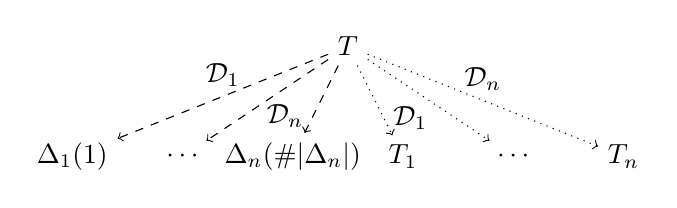
\begin{tikzpicture}[scale=0.7]
      % Nodes: Types
      \node (T) at (0,2) { $T$ };
      \node (T1) at (-5,0) { $\Delta_{1}(1)$ };
      \node (Tcdots1) at (-3,0) { $\cdots$ };
      \node (T2) at (-1,0) { $\Delta_{n}(\#\vert \Delta_{n} \vert)$ };
      \node (T3) at (1,0) { $T_{1}$ };
      \node (Tcdots2) at (3,0) { $\cdots$ };
      \node (T4) at (5,0) { $T_{n}$ };
      % Arrows: level a to b
      \draw[dashed,->] (T) -> (T1) node[midway,above] { $\mathcal{D}_{1}$ };
      \draw[dashed,->] (T) -> (Tcdots1);
      \draw[dashed,->] (T) -> (T2) node[near end,left] { $\mathcal{D}_{n}$ };
      \draw[dotted,->] (T) -> (T3) node[near end,right] { $\mathcal{D}_{1}$ };
      \draw[dotted,->] (T) -> (Tcdots2);
      \draw[dotted,->] (T) -> (T4) node[midway,above] { $\mathcal{D}_{n}$ };
    \end{tikzpicture}
    \caption{Type-graph building block for codata declaration.}
    \label{fig:mainideas:codatatg:tg}
  \end{subfigure}
  \caption{Codata.}
  \label{fig:mainideas:codatatg}
\end{figure}

Even forgetting the constructor/destructor labels $\mathcal{C}_{i}$ and $\mathcal{D}_{i}$ while retaining only the information:
\begin{enumerate}
  \item
    \enquote{constructor domain} (solid arrow)
  \item
    \enquote{destructor domain} (dashed arrow)
  \item
    \enquote{destructor codomain} (dotted arrow)
\end{enumerate}
still contains most type information.
We call the resulting graph \textit{reduced type-graph}.
\\
The reduced type-graph suffices to classify mutually recursive type definitions by the sort of the cycles it contains.
We only make the rough distinction that a cycle is \textit{recursively malign} if it contains a dashed edge while other cycles are \textit{recursively benign}.
Then we say that a program is \textit{strictly positive} if its reduced type-graph does not have recursively malign cycles.
This generalizes the ordinary formualtion of strict positivity where only codata types modeling an ordinary function type are allowed.

\subsubsection{SC}

The SC is a refinement of the PBC and hence the results of the previous discussion regarding strict positivity translate to the SC.
In fact, since there is a judgement $\con$ for refutations $X \rightarrow \bot$ now, it is not necessary to use a seperate type for continuations to encode the Curry paradox.
The producers of the type $\Curry$ are now precisely the consumers of it, making the inconsistency even more explicit.
On top, due to the symmetry of the SC, we get the dual of the Curry paradox for free.
Non-terminating commands are $\MakeExe(\run()) \mkCmd \run()$ and, dually, $\corun() \mkCmd \CoMakeExe(\corun())$.

\begin{minipage}{0.45\textwidth}
  \begin{codealign}
    % Curry datatype
    &
      \polprd\ \type\ \Curry\ \where
    \\[-4pt]
    &\quad
      \MakeExe(k \con \Curry)
    \\
    % run function
    &
      \define\
      \run() \con \Curry
      \coloneq
      \match
    \\[-4pt]
    &\quad
      \MakeExe(k \con \Curry) \Rightarrow \MakeExe(k) \mkCmd k
    \\
  \end{codealign}
\end{minipage}
\begin{minipage}{0.45\textwidth}
  \begin{codealign}
    % CoCurry codatatype
    &
      \polcon\ \type\ \CoCurry\ \where
    \\[-4pt]
    &\quad
      \CoMakeExe(x \prd \CoCurry)
    \\
    % corun function
    &
      \define\
      \corun() \prd \CoCurry
      \coloneq
      \match
    \\[-4pt]
    &\quad
      \CoMakeExe(x \prd \CoCurry) \Rightarrow x \mkCmd \CoMakeExe(x)
    \\
  \end{codealign}
\end{minipage}

Reduced type-graph are now built from the basic building blocks for $\polprd$ and $\polcon$ types as illustrated in \cref{fig:mainideas:prdtg} and \cref{fig:mainideas:contg}.
Note that while we still can forget the names but have to retain the information if it is a producer or a consumer as it is the key information in the Curry paradox.
This results in an orientation label $\pol$ and four sorts of edges:
\begin{enumerate}
  \item
    \enquote{producer in constructor domain} (dashed arrow labeld $\polprd$)
  \item
    \enquote{consumer in constructor domain} (dashed arrow labeld $\polcon$)
  \item
    \enquote{producer in destructor domain} (dotted arrow labeld $\polprd$)
  \item
    \enquote{consumer in destructor domain} (dotted arrow labeld $\polcon$)
\end{enumerate}

\begin{figure}[H]
  \begin{subfigure}[b]{0.25\textwidth}
    \begin{codealign}
      % T datatype
      &
        \polprd\ \type\ T\ \where
      \\[-4pt]
      &\quad
        \mathcal{X}_{1} \Delta_{1}
      \\[-4pt]
      &\quad\quad
        \vdots
      \\[-4pt]
      &\quad
        \mathcal{X}_{n} \Delta_{n}
    \end{codealign}
    \caption{$\polprd$ type declaration.}
    \label{fig:mainideas:prdtg:prdt}
  \end{subfigure}
  \begin{subfigure}[b]{0.7\textwidth}
    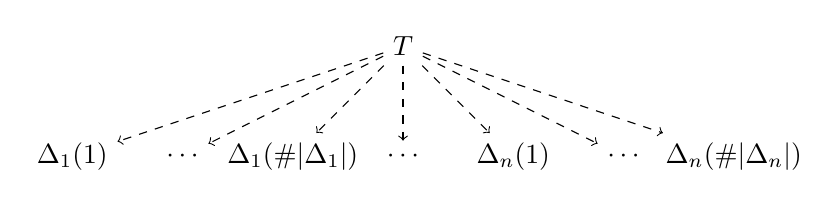
\begin{tikzpicture}[scale=0.7]
      % Nodes: types
      \node (T) at (0,2) { $T$ };
      \node (T1) at (-6,0) { $\Delta_{1}(1)$ };
      \node (Tcdots1) at (-4,0) { $\cdots$ };
      \node (T2) at (-2,0) { $\Delta_{1}(\#\vert \Delta_{1} \vert)$ };
      \node (Tcdots2) at (0,0) { $\cdots$ };
      \node (T3) at (2,0) { $\Delta_{n}(1)$ };
      \node (Tcdots3) at (4,0) { $\cdots$ };
      \node (T4) at (6,0) { $\Delta_{n}(\#\vert \Delta_{n} \vert)$ };
      % Arrows: level a to b
      \draw[dashed,->] (T) -> (T1) node[midway,above] { $\pol$ };
      \draw[dashed,->] (T) -> (Tcdots1);
      \draw[dashed,->] (T) -> (T2) node[midway,below] { $\pol$ };
      \draw[dashed,->] (T) -> (Tcdots2);
      \draw[dashed,->] (T) -> (T3) node[midway,below] { $\pol$ };
      \draw[dashed,->] (T) -> (Tcdots3);
      \draw[dashed,->] (T) -> (T4) node[midway,above] { $\pol$ };
    \end{tikzpicture}
    \caption{Reduced type-graph building block for $\polprd$ type declaration.}
    \label{fig:mainideas:prdtg:tg}
  \end{subfigure}
  \caption{$\polprd$ type.}
  \label{fig:mainideas:prdtg}
\end{figure}

\begin{figure}[H]
  \begin{subfigure}[b]{0.25\textwidth}
    \begin{codealign}
      % T codatatype
      &
        \polcon\ \type\ T\ \where
      \\[-4pt]
      &\quad
        \mathcal{X}_{1} \Delta_{1}
      \\[-4pt]
      &\quad\quad
        \vdots
      \\[-4pt]
      &\quad
        \mathcal{X}_{n} \Delta_{n}
    \end{codealign}
    \caption{$\polcon$ type declaration.}
    \label{fig:mainideas:contg:cont}
  \end{subfigure}
  \begin{subfigure}[b]{0.7\textwidth}
    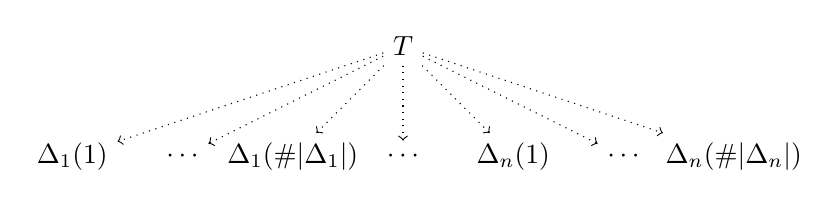
\begin{tikzpicture}[scale=0.7]
      % Nodes: types
      \node (T) at (0,2) { $T$ };
      \node (T1) at (-6,0) { $\Delta_{1}(1)$ };
      \node (Tcdots1) at (-4,0) { $\cdots$ };
      \node (T2) at (-2,0) { $\Delta_{1}(\#\vert \Delta_1 \vert)$ };
      \node (Tcdots2) at (0,0) { $\cdots$ };
      \node (T3) at (2,0) { $\Delta_{n}(1)$ };
      \node (Tcdots3) at (4,0) { $\cdots$ };
      \node (T4) at (6,0) { $\Delta_{n}(\#\vert \Delta_{n} \vert)$ };
      % Arrows: level a to b
      \draw[dotted,->] (T) -> (T1) node[midway,above] { $\pol$ };
      \draw[dotted,->] (T) -> (Tcdots1);
      \draw[dotted,->] (T) -> (T2) node[midway,below] { $\pol$ };
      \draw[dotted,->] (T) -> (Tcdots2);
      \draw[dotted,->] (T) -> (T3) node[midway,below] { $\pol$ };
      \draw[dotted,->] (T) -> (Tcdots3);
      \draw[dotted,->] (T) -> (T4) node[midway,above] { $\pol$ };
    \end{tikzpicture}
    \caption{Reduced type-graph building block for $\polcon$ type declaration.}
    \label{fig:mainideas:contg:tg}
  \end{subfigure}
  \caption{$\polcon$ type.}
  \label{fig:mainideas:contg}
\end{figure}

Eventually, the Curry paradox motivates the definition that a cycle is \textit{recursively malign} if it contains a dashed edge labeled $\polcon$ or, dually, a dotted edge labeled $\polprd$ and \textit{recursively benign} otherwise.
Again, we say that a program is \textit{strictly positive} if its reduced type-graph does not have recursively malign cycles.

\subsection{Structural Recursion}
\label{sec:mainideas:sr}

If a function somehow calls itself, then it is said to be recursive.
If moreover the argument of the recursive call is a part of the actual function argument, the recursion is said to be structural.
This constitutes a rough definition of structural recursion.
\\
Essentially, it tells us that a way to decide if a recursion is structural is to chase argument sizes through the call graph of a program and check if the sizes decrease when going through cycles.
In fact, \cite{foetus} develops a technique based on graphs, order relations and algebra doing that.
It is applicable to languages with data and pattern matching and in the following we show how to also adapt it to the SC.
\\
\\
First of all, applying \cite{foetus} necessarily requires order relations
\begin{enumerate}
  \item
    $t_{1} < t_{2}$: $t_{1}$ is structurally smaller than $t_{2}$
  \item
    $t_{1} \leq t_{2}$: $t_{2}$ is structurally not bigger than $t_{2}$
  \item
    $t_{1} \, ? \, t_{2}$: it is unknown how $t_{1}$ and $t_{2}$ relate (the catch-all case)
\end{enumerate}
on terms $t_{1}, t_{2}$ making up a rig $R :=( \{ <,\leq,? \},+,\cdot )$ by the binary operators $+$ (parallel combination) and $\cdot$ (serial combination) defined on $\{ <,\leq,? \}$:

\begin{figure}[H]
  \begin{subfigure}[t]{0.3\textwidth}
    \scriptsize
    \begin{tabular}{c|ccc}
        $+$
      & $<$
      & $\leq$
      & $?$
      \\
      \hline
        $<$
      & $<$
      & $<$
      & $<$
      \\
        $\leq$
      & $<$
      & $\leq$ &
      $\leq$
      \\
        $?$
      & $<$
      & $\leq$
      & $?$
      \\
    \end{tabular}
  \end{subfigure}
  \begin{subfigure}[t]{0.3\textwidth}
    \scriptsize
    \begin{tabular}{c|ccc}
        $\cdot$
      & $<$
      & $\leq$
      & $?$
      \\
      \hline
        $<$
      & $<$
      & $<$
      & $?$
      \\
        $\leq$
      & $<$
      & $\leq$
      & $?$
      \\
        $?$
      & $?$
      & $?$
      & $?$
      \\
    \end{tabular}
  \end{subfigure}
\end{figure}

This is because being a rig allows for matrix multiplication of matrices $M : \mathbb{N}_{n_{1}} \times \mathbb{N}_{n_{2}} \to R$ in the usual way.
\\
The idea then is to label the edges of the call graph with such matrices to track size changes of arguments between caller and callee (where $n_{1}$ is the arity of the caller and $n_{2}$ is the arity of the callee).
Because the rig $R$ is defined in such a way that composition of edges corresponds to matrix multiplication one can assign a size-matrix to each cycle and define structural recursion in terms of the diagonal of the matrix which contains the size changes of the arguments.
\\
\\
So what we need to make the approach work for the SC are only the respective definitions of the order relation as we already have a notion of call graph for the SC (we already defined what \enquote{calls} and \enquote{bodies} are).
And a simple possible generation of $<$, $\leq$ and $?$ for the SC ensuring well-foundedness w.r.t. the strict positivity from \cref{sec:mainideas:sp} is:
\begin{enumerate}
  \item
    Given variables $x_{1},\ldots,x_{n}$ and a producer/consumer $\mathcal{X}$ of some $\polprd$/$\polcon$ type then $x_{i} < \mathcal{X}(x_{1},\ldots,x_{n})$ for each producer/consumer $x_{i}$.
  \item
    Given a variable $x$ then $x \leq x$
  \item
    Given a variables $x_{1},x_{2}$ then $x_{1} \, ? \, x_{2}$
  \item
    \Authors{Note that we do not yet know if the previous generators are sufficient to ensure well-foundedness w.r.t. the strict positivity from \cref{sec:mainideas:sp}.}
\end{enumerate}
An SC program is then said to be \textit{structurally recursive} if the the entries from the \enquote{match-position} on the diagonal of the matrices assigned to the cycles are $<$.
And we are already done with structural recursion, actually.
\\
\\
Yet, to better understand the above let us look what all that means for the examples from \cref{fig:mainideas:SC:type:inductive} and \cref{fig:mainideas:SC:type:coinductive}.
The call graph of an SC program has a node for each match and a directed edge from a match to the machtes called in its bodies.
In both cases there is only one match - $\plus$ and $\const$, respectively.
$\plus$ calls nothing in the $\Zero$ case, but itself in the $\Succ$ case.
So there is on edge from $\plus$ to $\plus$ - a cycle.
Likewise, $\const$ calls nothing in the $\Head$ case, but itself in the $\Tail$ case and again there is one edge from $\const$ to $\const$.
\\
Relating the sizes of the arguments of the calls and gathering the result in matrices labeling the call graph yields:

\begin{figure}[H]
  \begin{subfigure}[t]{0.4\textwidth}
    \scriptsize
    \begin{tabular}{c|ccc}
        \diagbox{$\plus$}{$\plus$}
      & $\match$
      & $y \prd \Nat$
      & $k \con \Nat$
      \\
      \hline
        $\match$
      & $<$
      & $?$
      & $?$
      \\
        $y \prd \Nat$
      & $?$
      & $?$
      & $?$
      \\
        $k \con \Nat$
      & $?$
      & $?$
      & $\leq$
      \\
    \end{tabular}
  \end{subfigure}
  \begin{subfigure}[t]{0.4\textwidth}
    \scriptsize
    \begin{tabular}{c|cc}
        \diagbox{$\const$}{$\const$}
      & $\match$
      & $x \prd \Nat$
      \\
      \hline
        $\match$
      & $<$ & $?$
      \\
        $x \prd \Nat$
      & $?$ & $\leq$
      \\
    \end{tabular}
  \end{subfigure}
\end{figure}

Notably, the $<$ in the top left corner comes from the relations $x < \Succ(x)$ and $k < \Tail(k)$, respectively.
This shows that the relevant sizes (the one we match on) decrease when going through a cycle in these examples.
(And together with the well-foundedness of $<$ the size-change termination principle implies termination.)
\\
It also easily scales to more complicated programs like the SC implementation of subtraction derived from the (very economic) matrix presentation:

\begin{figure}[H]
  \begin{subfigure}[t]{0.5\textwidth}
    \scriptsize
    \begin{tabular}{c|cc}
        $\polprd\ \type\ \Nat$
      & $\Zero$
      & $\Succ(x \prd \Nat)$
      \\
      \hline
        $\sub(y \prd \Nat,k \con \Nat)$
      & $\Zero \mkCmd k$
      & $y \mkCmd \subaux(x,k)$
      \\
        $\subaux(y \prd \Nat,k \con \Nat)$
      & $\Succ(y) \mkCmd k$
      & $y \mkCmd \sub(x,k)$
      \\
    \end{tabular}
  \end{subfigure}
\end{figure}

Now there are nodes for $\sub$ and $\subaux$ as well as an edge from the former to the latter and vice versa.
The matrices labeling these edges are the same and multiplying the matrices shows that going through a cycle with basepoint $\sub$ structurally decreases the argument $\sub$ matches on:

\begin{figure}[H]
  \begin{subfigure}[t]{0.5\textwidth}
    \scriptsize
    \begin{tabular}{c|ccc}
        \diagbox{$\sub(\subaux$)}{$\subaux(\sub)$}
      & $\match$
      & $y \prd \Nat$
      & $k \con \Nat$
      \\
      \hline
        $\match$
      & $?$
      & $<$
      & $?$
      \\
        $y \prd \Nat$
      & $\leq$
      & $?$
      & $?$
      \\
        $k \con \Nat$
      & $?$
      & $?$
      & $\leq$
      \\
    \end{tabular}
  \end{subfigure}
  \begin{subfigure}[t]{0.4\textwidth}
    \scriptsize
    \begin{tabular}{c|ccc}
        \diagbox{$\sub$}{$\sub$}
      & $\match$
      & $y \prd \Nat$
      & $k \con \Nat$
      \\
      \hline
        $\match$
      & $<$
      & $?$
      & $?$
      \\
        $y \prd \Nat$
      & $?$
      & $<$
      & $?$
      \\
        $k \con \Nat$
      & $?$
      & $?$
      & $\leq$
      \\
    \end{tabular}
  \end{subfigure}
\end{figure}

(Again, together with the well-foundedness of $<$ the size-change termination principle implies termination.)
\\
In general, checking for structural recursion is only a matter of checking if the matrices labeling cycles have $<$ in the right place: the match position.

\subsection{Soundness}
\label{sec:mainideas:sound}

\Authors{This \cref{sec:mainideas:sound} is the open question.}
